\chapter{State of the Art}
\label{cha:soa}
The application of DL to planetary science is a rapidly expanding field.
As the volume and diversity of data returned by orbital missions continue to increase, traditional manual analysis methods are becoming progressively less scalable and more time consuming.
This chapter reviews the current state of the art in DL applied to planetary exploration, with a specific focus on RS data analysis and the use of Generative Adversarial Networks (GANs) and related architectures for signal processing, image enhancement, and Simulation-to-Real (Sim-to-Real) domain adaptation~\cite{yebasse2025advances}.

\section{Deep Learning in Planetary Science}
\label{sec:ml_planetary}
Historically, the analysis of planetary data has been driven by expert interpretation.
Geologists and geophysicists manually inspect images, optical and hyperspectral images, and radargrams to identify features of interest.
However, in the last decade, the availability of large-scale orbital datasets (e.g., HiRISE, CTX, CRISM, SHARAD, MARSIS) and advances in DL have led to a progressive shift towards automated methods based on convolutional and transformer-based architectures~\cite{Ronneberger_2015,He_2016}.

One of the earliest and most successful applications of DL in planetary science is automated crater detection and crater counting on Mars and the Moon~\cite{Silburt2019,LunarCraterDLReview}.
Impact craters are fundamental chronometers for planetary surfaces, and CNN-based detectors have been trained to identify and classify craters on Mars~\cite{Silburt2019,DeepMarsGithub} and the Moon~\cite{LunarCraterDL,LunarCraterDLReview}, achieving human-level performance with orders-of-magnitude higher throughput than manual surveys.
Architectures derived from U-Net and Fully Convolutional Networks (FCNs) are now standard for segmenting geomorphological features such as dunes, channels, and volcanic flows~\cite{Fernandez2019DuneMapping,DeepDuneMapping} from high-resolution optical imagery (e.g., HiRISE, CTX), often coupled with residual backbones such as ResNet~\cite{He_2016}.

Beyond surface morphology, DL has been applied to a wide range of planetary and terrestrial remote sensing tasks, including:
\begin{itemize}
    \item \textbf{Feature detection vs. semantic segmentation of surface units:} DL models support both object-level detection of discrete features (e.g., impact craters, boulders) and full semantic segmentation of surface units (e.g., lava flows, sedimentary deposits, polar layered terrains) from multispectral and hyperspectral images~\cite{Silburt2019,Fernandez2019DuneMapping,Wang2019DeepMars}. In the former, detectors or instance-segmentation networks localize individual features, while in the latter encoder–decoder architectures learn to assign a geological class to each pixel, producing dense surface morphology maps.
    \item \textbf{Change detection} between multi-temporal observations, used to identify active processes such as dust storms, frost deposition, or landslides by comparing deep feature representations across time~\cite{Parajuli2020DustDL,FrontiersSandstorm_2022}.
    \item \textbf{Super-resolution and enhancement} of orbital imagery, where SRGAN-like models synthesize high-resolution views from lower-resolution sensors, improving the visibility of small-scale structures of interest~\cite{Ledig2017SRGAN,Li2022SRGANRemoteSensing}. 
\end{itemize}

These developments are directly relevant for this thesis because they illustrate how DL can (i) learn robust feature representations from complex, noisy planetary data and (ii) support downstream scientific tasks such as mapping, detection, and anomaly discovery~\cite{yebasse2025advances}.
In particular, the success of encoder–decoder architectures and generative models in optical and SAR remote sensing motivates their adaptation to RS radargrams, which share many of the challenges discussed in Section~\ref{sec:rs_challenges} (e.g., speckle noise, depth-dependent attenuation, surface clutter, and the strong anisotropy between range and along-track directions), despite being physically different from natural images~\cite{yebasse2025advances}.

\begin{figure}[t]
    \centering
    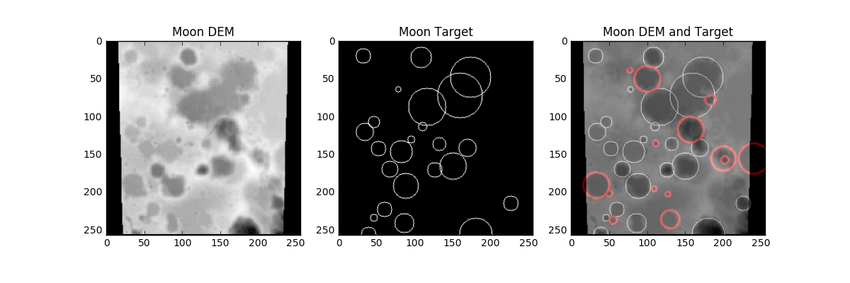
\includegraphics[width=0.75\textwidth]{images/dl_crater_segmentation}
    \caption{Example of DL-based crater detection and segmentation on planetary imagery. Convolutional encoder–decoder architectures, derived from U-Net, are widely used to detect and delineate impact craters, enabling large-scale, automated chronologic analysis. Reproduced from~\cite{Silburt2019}.}
    \label{fig:dl_crater_segmentation}
\end{figure}

\begin{figure}[t]
    \centering
    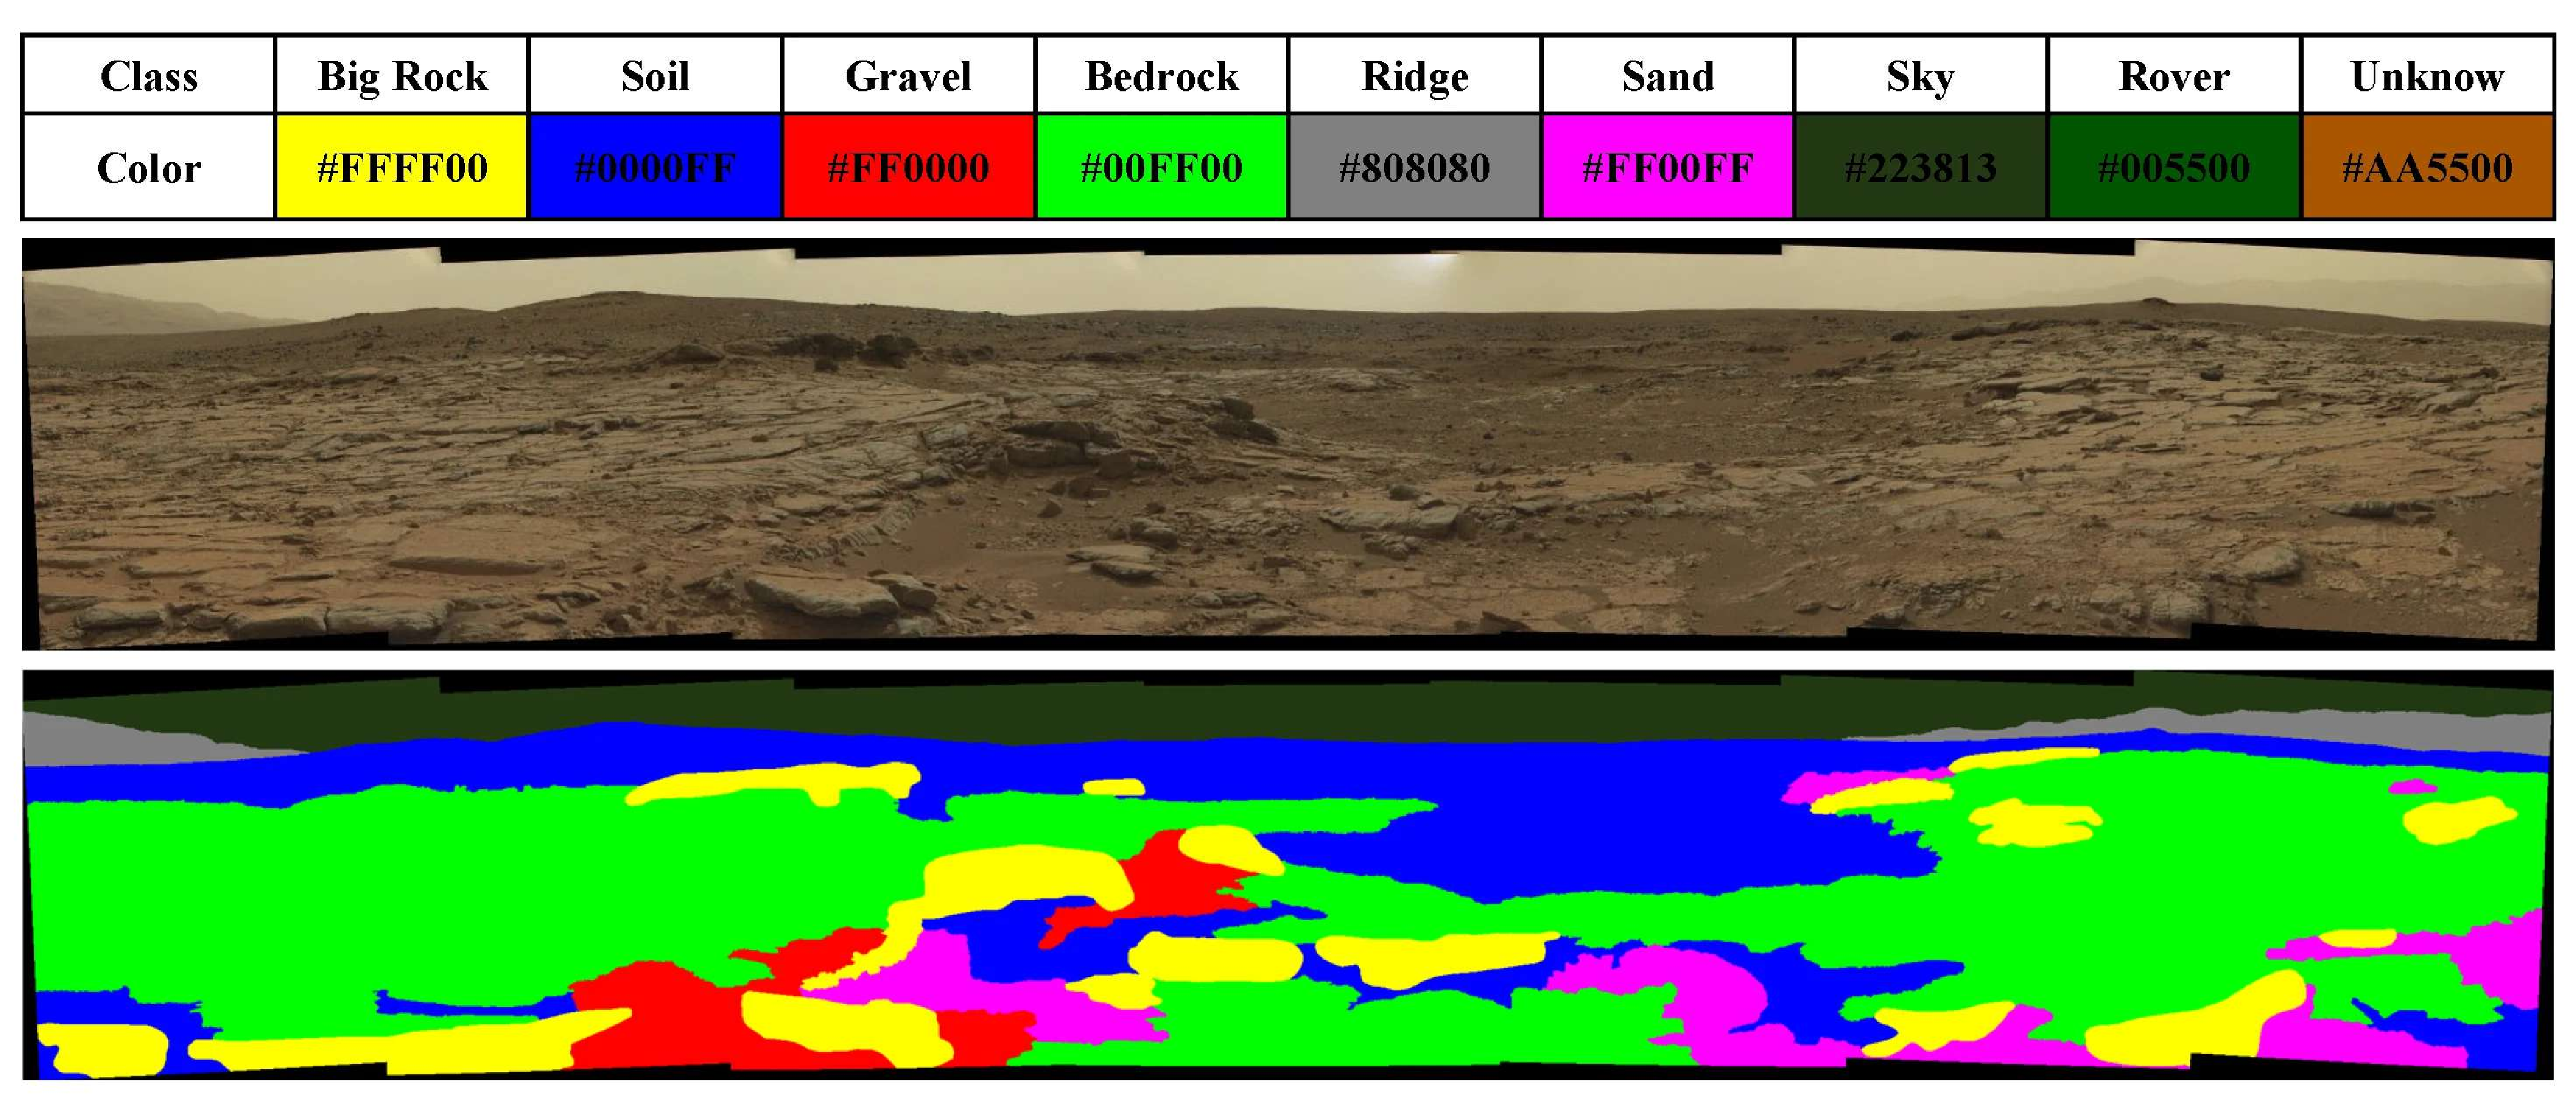
\includegraphics[width=0.85\textwidth]{images/dl_geomorph_mapping}
    \caption{Schematic illustration of DL-based geomorphological mapping from high-resolution orbital images. Semantic segmentation networks assign each pixel to a geomorphic class (e.g., lava flows, dunes, layered deposits), producing dense maps that support quantitative planetary surface studies. Example of terrain semantic segmentation reproduced from \cite{zhang2024s5mars}.}
    \label{fig:dl_geomorph_mapping}
\end{figure}


\section{Deep Learning for Radar Sounder Analysis}
\label{sec:dl_radar}
While DL has become a mature tool for optical and SAR Earth Observation, its application to Radar Sounder (RS) data (e.g., SHARAD, MARSIS) is more recent and poses unique challenges due to the non-intuitive nature of radargrams and the degradation mechanisms discussed in Section~\ref{sec:rs_challenges} (e.g., multiplicative speckle noise, depth-dependent dielectric attenuation, surface clutter, and the strong anisotropy between range and along-track directions)~\cite{Seu_2007,yebasse2025advances}.
Compared to natural images, RS data are closer to other coherent imaging modalities such as medical ultrasound or CT slices, where information is encoded in stratified structures and noisy, low-contrast interfaces rather than in visually recognizable objects~\cite{Daniels_2004,yebasse2025advances}.

In the broader remote sensing community, DL has already demonstrated its effectiveness for SAR despeckling, super-resolution, and style transfer.
GAN-based models are routinely employed to reduce speckle while preserving fine structures, to upsample SAR images beyond the native sensor resolution, and to perform domain adaptation between different sensors or acquisition conditions.
These successes provide a strong precedent for adopting similar architectures in the RS context, where the goal is to enhance radargrams, learn clutter statistics, and ultimately support tasks such as semantic segmentation, layer tracking, and anomaly detection.

Recent work on RS has started to adapt these ideas to the specific statistics and acquisition geometry of radargrams.
DL models have been proposed for semantic segmentation, layer tracking, denoising, super-resolution, and generative simulation of radargrams, often combining encoder–decoder architectures with adversarial or contrastive objectives to cope with limited labels and high noise levels.
In this thesis, the focus is on generative models for Sim-to-Real translation, which learn to map physically simulated radargrams into the style of real SHARAD observations while preserving subsurface structure.

\subsection{Numerical Simulators for Radar Sounding}
Numerical simulators play a central role in RS analysis, as they provide controllable, physics-based radargrams that can be used to interpret complex observations and to generate training data for DL models.
These simulators are broadly classified into two categories based on their treatment of wave propagation: \textbf{coherent} and \textbf{incoherent} models~\cite{Daniels_2004}.

\textbf{Coherent simulators} solve Maxwell's equations using full-wave methods such as finite-difference time-domain (FDTD) solvers.
These approaches capture phase information, interference patterns, multipath propagation, and frequency-dependent scattering, producing radargrams with physically accurate speckle statistics.
Tools like gprMax~\cite{Warren_2016} exemplify this class, enabling detailed simulation of complex subsurface geometries at the cost of significant computational expense.

\textbf{Incoherent simulators}, in contrast, model wave propagation as intensity-only processes, neglecting phase relationships.
Geometric optics ray-tracing is the most common approach: rays are traced from the radar platform to surface scatterers over Digital Elevation Models (DEMs), and incoherent power contributions are summed according to the radar equation.
This approximation is computationally efficient and produces realistic clutter patterns (hyperbolas, off-nadir surface returns) without speckle, making it suitable for rapid forward modeling and large-scale parametric studies~\cite{Seu_2007}.

In the context of this thesis, rather than developing a custom simulator, we utilized the surface clutter simulations used for SHARAD data and provided by the NASA Planetary Data System (PDS)~\cite{Choudhary_2016}.
These pre-computed synthetic radargrams are generated using an incoherent geometric-optics simulator that traces rays over Martian topographic data, specifically DEMs derived from the Mars Orbiter Laser Altimeter (MOLA)~\cite{Smith_2001} or the High Resolution Stereo Camera (HRSC)~\cite{Neukum_2004}, in order to predict the expected surface clutter for each specific SHARAD observation.
By providing a theoretical baseline of the surface scattering, these idealized radargrams serve as an optimal starting point for the Sim-to-Real generative models, enabling the network to learn realistic clutter textures and to isolate genuine subsurface anomalies.

\subsection{Radargram Denoising}
A primary focus of recent research has been the removal of noise and clutter to improve the interpretability of radargrams.
Traditional methods relied on band-pass filtering, wavelet transforms, or model-based clutter suppression; however, these often degrade the resolution of fine stratigraphic layers and may erase subtle reflectors of geological significance~\cite{Daniels_2004,yebasse2025advances}.
In particular, aggressive filtering can reduce speckle variance but simultaneously smear or suppress weak subsurface interfaces that are critical for geological interpretation.

DL-based approaches address these limitations by learning the noise and clutter statistics directly from data.
Autoencoders and CNN-based denoising networks are trained to reconstruct radargrams while suppressing background interference, effectively learning to separate coherent subsurface echoes from incoherent noise~\cite{yebasse2025advances}.
Generative models such as GANs and diffusion models have also been explored for radargram enhancement.
In analogy with SAR despeckling, adversarial training encourages the generator to produce outputs whose local texture and speckle patterns are statistically consistent with real data, avoiding the over-smoothed appearance typical of purely pixel-wise losses~\cite{Li2022SRGANRemoteSensing,Arjovsky2017}.
This is particularly relevant for the present work, where the goal is not merely to \enquote{clean} the radargrams, but to generate realistic realizations of clutter and noise that can serve as a reference background for residual-based anomaly detection~\cite{yebasse2025advances}.

\subsection{Layer Detection}
A parallel line of research focuses on automatic detection and tracking of subsurface horizons and discontinuities.
Classical approaches relied on edge detection and heuristic tracking along the along-track direction, often requiring substantial manual intervention by experts to correct missed or spurious picks~\cite{Daniels_2004,Seu_2007}.
Encoder–decoder architectures similar to U-Net have been used to perform pixel-wise detection of layer boundaries, replacing manual picking with fully automated horizon tracing~\cite{yebasse2025advances}.
In these models, skip connections ensure that thin, low-contrast reflectors are preserved, while deeper layers capture the broader stratigraphic context across tens to hundreds of range lines.

More recent work has introduced attention mechanisms and transformer-based models that explicitly exploit the long-range horizontal continuity of horizons across the azimuth direction, improving robustness to local noise and clutter disruptions~\cite{yebasse2025advances}.
These architectures treat the radargram as a sequence of range profiles and learn to propagate information along-track, allowing the network to maintain coherent horizon trajectories even in regions where the signal temporarily fades below the noise floor or is partially masked by surface clutter.

\subsection{Semantic Segmentation of Radargrams}
Beyond explicit horizon tracking, DL has also been applied to full semantic segmentation of radargrams, where each pixel is assigned to a geological or radiometric class (e.g., surface return, shallow layered unit, deep diffuse clutter, instrument noise)~\cite{yebasse2025advances}.
U-Net-like architectures trained on manually annotated radargrams or on hybrid simulation–observation datasets have been used to delineate continuous stratigraphic units and to separate subsurface interfaces from clutter-dominated regions, effectively extending surface geomorphological mapping concepts to the radargram domain.

In some studies, semantic segmentation networks are complemented by physically based simulators: geometric-optics or FDTD models provide synthetic labels for clutter-only scenarios, while real radargrams supply examples of mixed subsurface and clutter responses~\cite{Warren_2016,yebasse2025advances}.
This hybrid supervision strategy mitigates the scarcity of hand-labeled planetary RS data and enables the networks to learn class boundaries that are consistent with both radar physics and observed statistics.
Conceptually, horizon tracking and semantic segmentation form complementary views of the same problem: the former focuses on precise localization of individual reflectors, while the latter aims at assigning consistent classes to broader regions of the radargram, which can then be used as input or context for downstream anomaly detection and 3D reconstruction.

\subsection{The 3D Reconstruction Challenge}
Inferring the three-dimensional structure of the subsurface from two-dimensional radargrams is an ill-posed inverse problem, primarily due to surface clutter, unknown dielectric properties, and limited spatial coverage.
Off-nadir reflections can overlay valuable subsurface data, and the mapping between echo delay and physical depth depends on spatially varying permittivity.
Classical approaches rely on geometric-optics clutter simulations and the usage of multiple parallel acquisition tracks to form cross-track stacks and manual or semi-automatic interpretation to distinguish true subsurface interfaces from clutter, but fully automated 3D reconstruction remains a major open challenge~\cite{foss2017sharad3d,yebasse2025advances}.

DL offers several promising directions to tackle this problem.
One line of work uses CNNs or transformers to learn mappings from stacks of radargrams (or from radargram–topography pairs) to volumetric labels, effectively performing 3D semantic segmentation or horizon extraction in C-scan volumes~\cite{foss2017sharad3d,yebasse2025advances}.
Another direction exploits generative models trained on simulated clutter data to \enquote{inpaint} occluded regions, reconstructing the most likely continuation of subsurface layers beneath clutter masks~\cite{yebasse2025advances}.
In both cases, the success of the method depends critically on the availability of realistic simulations and on the ability of the network to learn physically plausible priors over subsurface geometries.

For planetary RS, these 3D approaches are still in their infancy, constrained by the limited availability of volumetric datasets and ground truth~\cite{foss2017sharad3d}.
Nonetheless, they highlight an important conceptual shift that is also embraced in this thesis: instead of treating each radargram independently, DL can be used to model the joint statistics of collections of radargrams and to leverage simulated data to regularize inherently ambiguous inversions~\cite{yebasse2025advances}.
The Sim-to-Real generative framework developed here can be seen as a first step in that direction, focusing on learning a robust background model of RS clutter against which truly anomalous subsurface responses can be detected~\cite{yebasse2025advances,Warren_2016}.


\section{Generative Models in Remote Sensing}
\label{sec:generative_rs}
Generative Adversarial Networks (GANs)~\cite{Goodfellow_2014} have found significant applications in Earth Observation, particularly with SAR and coherent imaging data.
These applications provide the direct inspiration for the methodology adopted in this thesis~\cite{Li2022SRGANRemoteSensing,yebasse2025advances}.

In the context of RS data, GANs offer an attractive framework for learning complex, high-dimensional distributions of radargrams without requiring explicit parametric models of clutter, speckle, or instrumental effects~\cite{yebasse2025advances}.
Instead of hand-crafting statistical models for each noise source, a GAN can be trained to reproduce the joint distribution of real RS observations conditioned on auxiliary inputs (e.g., simulations, masks), implicitly capturing the characteristic speckle patterns, amplitude statistics, and large-scale clutter geometries.
This flexibility comes at the cost of more delicate training dynamics, which motivates the careful choice of architectures and loss functions discussed in Chapter~\ref{cha:methodology}.

\subsection{Despeckling and Super-Resolution in Coherent Imaging}
SAR images, like radargrams, suffer from multiplicative speckle noise.
GAN-based models have demonstrated superior performance in despeckling compared to classical filters (e.g., Lee or Frost filters)~\cite{Ma2020SARGAN,Gu2019GANDespeckling}.
By employing a discriminator that judges texture realism, GANs can hallucinate high-frequency details that are statistically consistent with the terrain, rather than blurring them out.
This leads to outputs that are visually sharper and often more informative for downstream tasks such as classification or change detection~\cite{Li2022SRGANRemoteSensing}.

Furthermore, Super-Resolution GANs (SRGANs) have been applied to upsample low-resolution satellite imagery, enhancing the visibility of small-scale features~\cite{Ledig2017SRGAN,Li2022SRGANRemoteSensing}.
In SAR and RS contexts, such models can improve the apparent spatial resolution while preserving, or even accentuating, structural features like linear infrastructures, small water bodies, or fine topographic details~\cite{Donini2024SuperResRS}.
Recent work by Donini et al. (FBK, UniTn) specifically addresses super-resolution of radargrams, demonstrating that GANs can learn to recover fine stratigraphic details and reduce the impact of limited range resolution in planetary RS data~\cite{Donini2024SuperResRS}.

\subsection{Sim-to-Real Transfer}
A critical limitation in training DL models for planetary science is the scarcity of labeled \enquote{ground truth} data.
Unlike terrestrial applications where ground validation is feasible, planetary RS observations cannot be easily verified through in-situ measurements such as drill cores or geophysical surveys.
Even expert manual annotations remain subjective, inconsistent across interpreters, and fundamentally limited by the ambiguity inherent to radargram interpretation.
This paucity of reliable labels has motivated the development of \textbf{Simulation-to-Real (Sim-to-Real)} transfer learning approaches~\cite{Zhu_2017,yebasse2025advances}.

The workflow typically involves:
\begin{enumerate}
    \item Generating extensive synthetic datasets using physics-based simulators (e.g., FDTD Maxwell solvers or geometric optics clutter models) that provide complete control over subsurface geometry, dielectric properties, and acquisition parameters~\cite{Warren_2016}.
    \item Training models on this clean, fully labeled synthetic data, which includes ground truth for subsurface interfaces, clutter masks, and noise-free conditions.
    \item Adapting the model to solve tasks in the real domain.
\end{enumerate}

CycleGAN~\cite{Zhu_2017} and related architectures are particularly effective for this adaptation, as they learn to translate between \enquote{Clean Simulation} and \enquote{Noisy Real} domains without requiring perfectly aligned training pairs.
This enables \textbf{controlled data augmentation}: starting from a single simulated radargram, the network can generate multiple realistic variants that preserve the subsurface structure while introducing the full spectrum of real-world clutter statistics, speckle textures, and instrumental effects observed in SHARAD data~\cite{yebasse2025advances}.
The resulting augmented dataset bridges the sim-to-real domain gap, substantially improving model generalization to operational planetary RS observations.



\section*{Summary}
The methods reviewed in this chapter demonstrate the potential of DL and generative models for RS data enhancement, denoising, layer tracking, and 3D reconstruction.
However, existing approaches typically address these tasks independently and often rely on simplified assumptions about the relationship between simulated physics and real observations.
This motivates the Sim-to-Real generative framework and anomaly detection pipeline developed in this thesis, which are introduced in detail in Chapters~\ref{cha:methodology} and \ref{cha:results}.


